% !TeX encoding=utf8
% !TeX spellcheck = en-US

\chapter{Previous Work}
Recommender system literature can typically be divided into two categories: 1) content (or item) recommendation and 2) user recommendation. An example of content recommender systems is Amazon product recommendations. These take the form of "users who bought x also bought y".  An example of user recommendation is LinkedIn's "Do You Know..." feature, which is suggestingThe latter can be generalized as "Who To Follow" recommender systems and it is this type of recommendation on which this paper will focus.

\section{Recommendation As Link Prediction}
\begin{figure}[H]
  \centering
  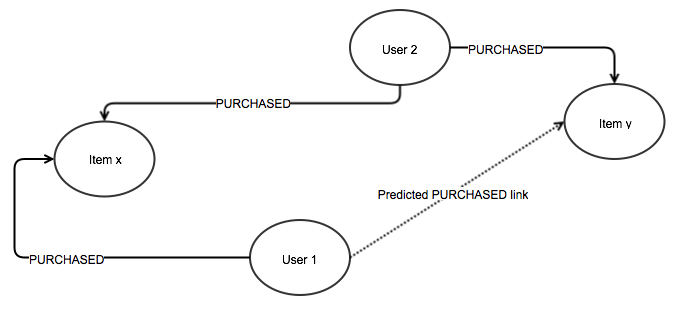
\includegraphics[width=0.75\textwidth]{images/item_link_prediction.png}
  \caption[Item Link Prediction]{Here we see an example of an item recommender system modeled as a graph where the nodes are Users and Items and the edges indicate a purchse of an Item by a User. When modeled this way recommendation takes the form a predicted link in the graph.}
  \label{fig:figures:1}
\end{figure}


\section{User-User Recommender Systems}
There are essentially two types of User-User recommender system algorithms: 1) Similarity based methods and 2) Network based methods.(CITATION NEEDED) Similarity based methods rely on the computation of a user-user similarity metric, which is then used to make recommendations. This is based on the homopholy principle, that users are more likely to be interested in users similar to them. Network based methods analyze the structure of the network to develop recommendations. Example include PageRank, HITS, and SALSA (CITATION NEEDED).

\subsection{Similarity Based Methods}

Collaborative filtering systems produce user specific recommendations based on patterns of behavior observed from other users. Typically this involves observing ratings of items and using either latent factor models or a neighborhood based approach to generate item recommendations\cite{cf}. With the rise of social network analysis however, often instead of user-item recommendations, we are more interested in generating user-user recommendations. User-user recommendations are the focus of this project. The underlying assumption of collaborative filtering is that of homophily: similar users like similar things. Collaborative filtering implementations can be problematic when applied to a large dataset. Most methods require a large sparse matrix for computation, the use of which is not always performant. Instead, the problem can be modeled as a graph, and make use of the graph traversal pattern as an alternative to the construction of a large sparse matrix \cite{Rodriguez}.

\subsection{Network Based Methods}

User-User recommender systems are often generalized as "Who To Follow" recommender systems, as made popular by the "Follow" social network action in the Twitter social network. A Follow action indicates a user expressing interest in another user in the network. This often involves 

The Twitter Who To Follow system is an example of a link prediction system running in production. \cite{wtf} details the design and implementation considerations for such a large scale system. The Twitter system operates on a custom in-memory graph processing engine which implements a PageRank-type algorithm known as Stochastic Approach for Link-Structure Analysis (SALSA). SALSA uses a random walk of the graph to generate link predictions.

\section{Directed Social Networks}
There is an important distinction to note between undirected social networks and directed social networks. Examples/explanation. Much of the literature has focused on undirected social networks only (CITATION NEEDED). In fact the similarity metrics shown above are all based on 